\documentclass[border=3pt]{standalone}
% Preâmbulo compartilhado pelos diagramas TikZ da aula 13 (SLAM com EKF)
\usepackage[T1]{fontenc}
\usepackage[utf8]{inputenc}
\usepackage{lmodern}
\usepackage{amsmath}
\usepackage{xcolor}
\usepackage{tikz}
\usetikzlibrary{arrows.meta,angles,quotes,decorations.pathmorphing,decorations.pathreplacing,calc,
                positioning,shapes.geometric,shapes.misc,backgrounds,fit,
                math}

% Paleta (mesma dos SVGs originais)
\definecolor{dblue}{HTML}{2A5B8C}
\definecolor{dorange}{HTML}{B3541E}
\definecolor{dgreen}{HTML}{4A7C59}
\definecolor{dred}{HTML}{9C4B4B}
\definecolor{dcream}{HTML}{F4F1EA}
\definecolor{dshade}{HTML}{DDD7C9}

% Função gaussiana (não normalizada por padrão de escala visual)
\pgfmathdeclarefunction{gauss}{3}{%
  \pgfmathparse{1/(#3*sqrt(2*pi))*exp(-((#1-#2)^2)/(2*#3^2))}%
}

% Estilos comuns (prefixo d... para não colidir com chaves internas do pgf)
\tikzset{
  >={Stealth[length=2mm]},
  dguide/.style={gray!55, dashed, line width=0.4pt},
  daxis/.style={gray!60, line width=0.7pt, ->},
  dbody/.style={fill=black!3, draw=black!80, line width=1pt},
  dacc/.style={draw=dblue, line width=1pt},
  dlbl/.style={black!55, font=\small},
  dsub/.style={black!45, font=\footnotesize},
  dstate/.style={circle, draw=black!80, fill=dcream, line width=1pt,
                 minimum size=17mm, font=\large, inner sep=1pt},
  dobs/.style={circle, draw=black!80, fill=dshade, line width=1pt,
               minimum size=14mm, font=\large, inner sep=1pt},
  dbox/.style={rounded corners=2pt, draw=black!80, fill=dcream, line width=1pt,
               align=center, inner sep=6pt},
  dop/.style={circle, draw=black!80, fill=white, line width=1pt,
              minimum size=6mm, inner sep=0pt, font=\small},
  dtrans/.style={->, dblue, line width=1pt},
  dmeas/.style={->, dorange, line width=1pt},
  dcurve/.style={line width=1pt, dblue},
  dcurveb/.style={line width=1.4pt, dorange},
}

\begin{document}
\hyphenpenalty=10000 \exhyphenpenalty=10000 \tolerance=9999 \emergencystretch=3em
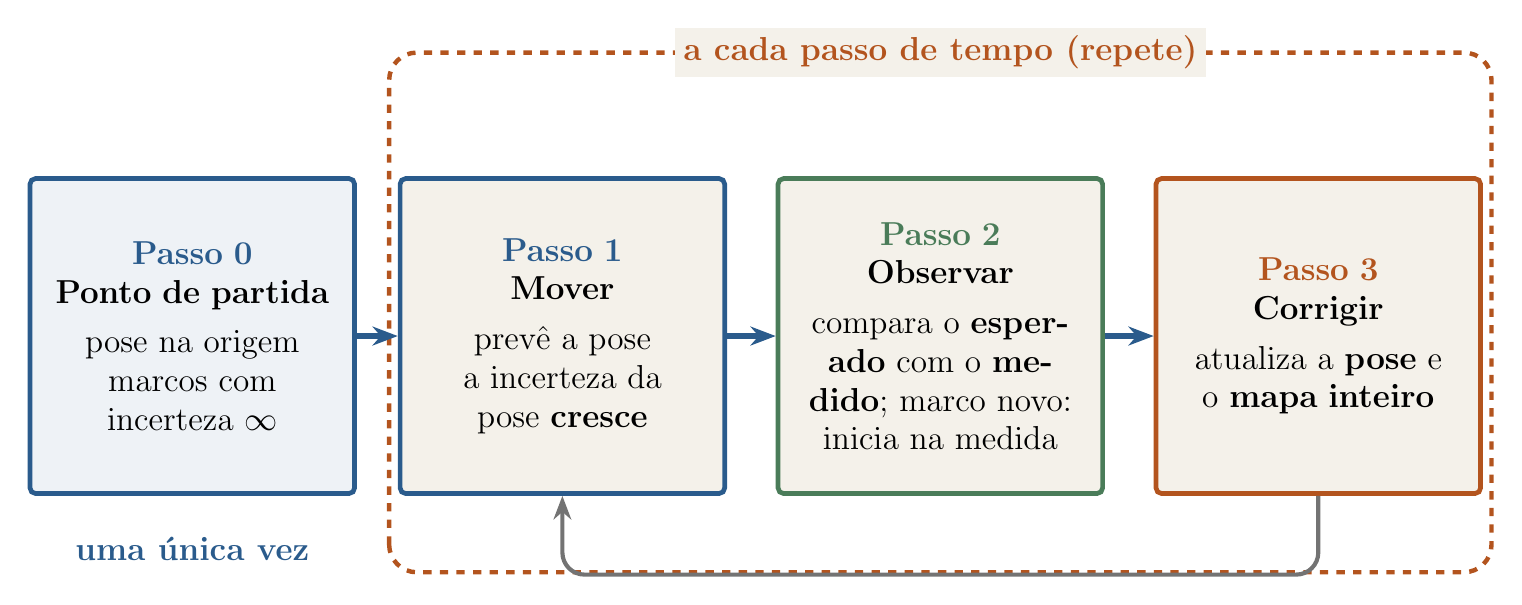
\begin{tikzpicture}[x=1cm,y=1cm]
\tikzset{c/.style={dbox, text width=3.7cm, minimum height=4.0cm, font=\large, line width=1.7pt},
        a/.style={dtrans, line width=2pt, -{Stealth[length=3.2mm]}}}
\node[c, draw=dblue, fill=dblue!8] (p0) at (2.5,4.3) {\textbf{\textcolor{dblue}{Passo 0}}\\ \textbf{Ponto de partida}\\[4pt] pose na origem\\ marcos com incerteza $\infty$};
\node[font=\large\bfseries, dblue] at (2.5,1.6) {uma única vez};
\draw[dorange, dashed, line width=1.6pt, rounded corners=10pt] (5.0,1.3) rectangle (19.0,7.9);
\node[font=\large\bfseries, dorange, fill=dcream, inner sep=3pt] at (12.0,7.9) {a cada passo de tempo (repete)};
\node[c, draw=dblue] (p1) at (7.2,4.3) {\textbf{\textcolor{dblue}{Passo 1}}\\ \textbf{Mover}\\[4pt] prevê a pose\\ a incerteza da pose \textbf{cresce}};
\node[c, draw=dgreen] (p2) at (12.0,4.3) {\textbf{\textcolor{dgreen}{Passo 2}}\\ \textbf{Observar}\\[4pt] compara o \textbf{esperado} com o \textbf{medido}; marco novo: inicia na medida};
\node[c, draw=dorange] (p3) at (16.8,4.3) {\textbf{\textcolor{dorange}{Passo 3}}\\ \textbf{Corrigir}\\[4pt] atualiza a \textbf{pose} e o \textbf{mapa inteiro}};
\draw[a] (p0.east) -- (p1.west);
\draw[a] (p1.east) -- (p2.west);
\draw[a] (p2.east) -- (p3.west);
\draw[black!55, line width=1.5pt, -{Stealth[length=3mm]}, rounded corners=8pt] (p3.south) -- ++(0,-1.0) -| (p1.south);
\end{tikzpicture}
\end{document}
